%Constitution of Linguistics Society, AAHKUSU
%Source code
%Typeset in \LaTeX by Chik Wing Cheung Aaron, Academic Officer and Publication Officer, Linguistics Society, AAHKUSU, Session 2017--2018

%Basic packages
\documentclass[11pt,a4paper,notitlepage]{article}
\usepackage[left=2.50cm, right=2.50cm, top=2.50cm, bottom=2.50cm]{geometry}
\usepackage[utf8]{inputenc}
\usepackage[UKenglish]{babel}
\usepackage{graphicx}
\usepackage{ulem}
\usepackage[explicit]{titlesec}
\usepackage{enumitem}
\usepackage{appendix}



%Set typefaces
\usepackage{luatexja-fontspec}
\setmainjfont{Noto Serif CJK KR Medium}
%\setmainfont[Ligatures=TeX]{Times LT Std}
\setmainfont[Ligatures=TeX]{Charis SIL}
\newfontfamily\arialnarrow[Ligatures=TeX]{Arial Nova Cond Bold}



%Disable hyphenation, no matter how ugly the output looks
\tolerance=1
\emergencystretch=\maxdimen
\hyphenpenalty=10000
\hbadness=10000

%Redefine section heading
\makeatletter
\def\section{\@ifstar\unnumberedsection\numberedsection}
\def\numberedsection{\@ifnextchar[%]
	\numberedsectionwithtwoarguments\numberedsectionwithoneargument}
\def\unnumberedsection{\@ifnextchar[%]
	\unnumberedsectionwithtwoarguments\unnumberedsectionwithoneargument}
\def\numberedsectionwithoneargument#1{\numberedsectionwithtwoarguments[#1]{#1}}
\def\unnumberedsectionwithoneargument#1{\unnumberedsectionwithtwoarguments[#1]{#1}}
\def\numberedsectionwithtwoarguments[#1]#2{%
	\ifhmode\par\fi
	\removelastskip
	\vskip 3ex\goodbreak
	\refstepcounter{section}%
	\begingroup
	\noindent\leavevmode\Large\centering 
	Section \thesection\ \\ \uline{\textsc{\textbf{#2}}}\par
%	\textit{\MakeUppercase{Section \thesection}} \\ \uline{\textsc{#2}}\par
	\endgroup
	\vskip 2ex\nobreak
	\addcontentsline{toc}{section}{%
		\protect\numberline{\thesection}%
		#1}%
}
\def\unnumberedsectionwithtwoarguments[#1]#2{%
	\ifhmode\par\fi
	\removelastskip
	\vskip 3ex\goodbreak
	%  \refstepcounter{section}%
	\begingroup
	\noindent\leavevmode\Large\bfseries\centering 
	%  \S \thesection\ 
	#2\par
	\endgroup
	\vskip 2ex\nobreak
	\addcontentsline{toc}{section}{%
		%    \protect\numberline{\thesection}%
		#1}%
}
\def\subsection{\@ifstar\unnumberedsubsection\numberedsubsection}
\def\numberedsubsection{\@ifnextchar[%]
	\numberedsubsectionwithtwoarguments\numberedsubsectionwithoneargument}
\def\unnumberedsubsection{\@ifnextchar[%]
	\unnumberedsubsectionwithtwoarguments\unnumberedsubsectionwithoneargument}
\def\numberedsubsectionwithoneargument#1{\numberedsubsectionwithtwoarguments[#1]{#1}}
\def\unnumberedsubsectionwithoneargument#1{\unnumberedsubsectionwithtwoarguments[#1]{#1}}
\def\numberedsubsectionwithtwoarguments[#1]#2{%
	\ifhmode\par\fi
	\removelastskip
	\vskip 3ex\goodbreak
	\refstepcounter{subsection}%
	\begingroup
	\noindent\leavevmode\Large\bfseries\centering 
	Subsection \thesubsection\ \\ \uline{\textsc{#2}}\par
	\endgroup
	\vskip 2ex\nobreak
	\addcontentsline{toc}{subsection}{%
		\protect\numberline{\thesubsection}%
		#1}%
}
\def\unnumberedsubsectionwithtwoarguments[#1]#2{%
	\ifhmode\par\fi
	\removelastskip
	\vskip 3ex\goodbreak
	%  \refstepcounter{subsection}%
	\begingroup
	\noindent\leavevmode\Large\bfseries\centering 
	%  \S \thesubsection\ 
	#2\par
	\endgroup
	\vskip 2ex\nobreak
	\addcontentsline{toc}{subsection}{%
		%    \protect\numberline{\thesubsection}%
		#1}%
}
\makeatother
%End of section redefinition


%Disable section and subsection numbering in paragraphs
\renewcommand{\thesubsection}{\hspace*{-1.0em}}
\renewcommand{\thesubsubsection}{\hspace*{-1.0em}}
\renewcommand{\theparagraph}{\arabic{paragraph}}

%Define paragraph numbering and label. All articles are automatically numbered and not indented.
\setcounter{secnumdepth}{4}
\titleformat{\paragraph}[display]
{\normalfont\normalsize\bfseries}{}{0pt}{Article \theparagraph:\space#1}{}
\titlespacing*{\paragraph}{0pt}{0pt}{0pt}

%Suppress page numbering
%\pagestyle{empty}



%\title{
\includegraphics[height=4cm]{graphics/logotype_spec_1}\\
\title{
\includegraphics[height=4cm]{graphics/logo-PDF_GreyscaleLogoonLight}\\
	\textbf{Constitution of Linguistics Society, AAHKUSU}}
\date{}


%Redefine appendices to appendix
\renewcommand*\appendixpagename{Appendix}
\renewcommand*\appendixtocname{Appendix}


%Annotation mark -- do not remove


\pagestyle{headings}
\markright{{\arialnarrow\small \textup{\MakeUppercase{(Annotated copy)} For printing only. Annotations not part of the Constitution -- refer to the official document.}}}

\author{\arialnarrow \MakeUppercase{Annotated copy}}

\usepackage{draftwatermark}
\SetWatermarkText{{\arialnarrow \MakeUppercase{Annotated}}}
\SetWatermarkScale{0.5}

%The content of the Constitution begins below
\begin{document}
	%Suppress page number on title page
	\pagenumbering{gobble}
	\maketitle
	\section{Interpretation}
	\paragraph{} ``University'' shall mean The University of Hong Kong.
	
	\paragraph{} ``HKUSU'' shall mean the Hong Kong University Students' Union.
	
	\paragraph{} ``Department'' shall mean the Department of Linguistics, School of Humanities, Faculty of Arts, The University of Hong Kong.
	
	\paragraph{} ``AAHKUSU'' shall mean the Arts Association, Hong Kong University Students' Union.
	
	\paragraph{} ``Society'' shall mean Linguistics Society, AAHKUSU.
	
	\paragraph{} ``Committee'' shall mean the Executive Committee of Linguistics Society, AAHKUSU. 
	
	\paragraph{} ``Members'' shall mean the members of Linguistics Society, AAHKUSU. 
	
	\paragraph{} ``Constitution'' shall mean the Constitution of Linguistics Society, AAHKUSU. 
	
	\paragraph{} ``President'' shall mean the President of the Executive Committee of Linguistics Society, AAHKUSU.
	
	\paragraph{} ``General Meeting'' shall include the Annual General Meeting (AGM), and any Extraordinary General Meeting (EGM) of the Society. 
	
	\paragraph{} ``Undergraduates'' shall mean students of The University of Hong Kong who are taking full-time undergraduate degree course(s). 
	
	\paragraph{} ``Clear day'' shall mean a complete day of 24 hours; and ``clear days'' shall mean a period of complete days, excluding the intervening public holidays. 
	
	
	\section{Constitution} 
	
	\paragraph{Interpretation}
	The Committee shall have the sole right of interpretation of the Constitution during its session of office. 
	
	\paragraph{Alteration and Amendment}
	No alteration or amendment of the Constitution may be made except at the General Meetings convened for that purpose, notice intimating specially the changes proposed of which shall have been posted at least 6 clear days in advance. 
	
	\paragraph{Motions}
	A motion to alter or amend any part of the Constitution shall be carried only when so agreed to by not less than two-third of the members present and voting at that General Meeting. 
	
	\paragraph{Reference}
	In case of dispute for which no ruling has been given in the Constitution, reference should be made to the Constitution of the Arts Association, HKUSU and to the Constitution of the Hong 
	Kong University Students' Union. 
	
	
	\section{General}
	
	\paragraph{Name}
		\begin{enumerate}
			\item The name of the Society in English shall be ``Linguistics Society, AAHKUSU''. 
			\item The name of the Society in Chinese shall be ``香港大學學生會文學院學生會語言學學會''. 
		\end{enumerate}
	
	
	\paragraph{Purposes and Aims} 
	The purposes and aims of the Society shall be: 
	\begin{enumerate}
		\item To promote the complete organisation and unity within the Society. 
		\item To promote the general welfare of Members. 
		\item To promote the better understanding among Members and the teaching staff of Department. 
		\item To promote the academic interests of Members. 
		\item To represent the interests of Members. 
	\end{enumerate}
	
	\paragraph{Society Session} 
	The Society session shall commence at the conclusion of the AGM and shall terminate at the conclusion of the AGM in the following year. 
	
	\paragraph{Management} 
	The management of the Society during the session of office shall be vested in the Committee as elected in accordance with the provision of the Constitution. 
	
	\paragraph{Official Languages} 
	English and Chinese shall be the official languages of the Society in either or both of which all official meetings and official correspondence shall be conducted. Chinese, in its oral form, shall mean the Cantonese dialect and Mandarin. 
	
	\paragraph{Affiliation} 
	The Society shall be an academic society affiliated to the Arts Association, Hong Kong University Students' Union. 
	 
	\paragraph{Motto}
	The motto of the Society shall be ``\textit{ad linguisticam promovendam}''.
	
	\paragraph{Logotype}
	The logotype of the Society shall be as defined in Appendix I.
	
	 
	\section{Membership} 
	
	\paragraph{Definitions} 
	\begin{enumerate}
		\item Honorary Membership \par
		All teaching staff of Department and graduated ex-members of the Committee shall be Honorary Members, except those who are dismissed under Section 5, Article 8(2). 
		\item Full Membership \par
		Undergraduates taking or enrolled in any course(s) of the Department in the same academic year shall be Full Members after paying the prescribed membership fee.
		\item Affiliate Membership \par
		Undergraduates taking or enrolled in any course(s) of the Department in the same academic year shall be Affiliate Members. 
		\item Associate Membership \par
		Undergraduates who are not taking courses of the Department shall be Associate Members after paying the prescribed membership fee. 
	\end{enumerate}
	
	\paragraph{Privileges of Members}
	\begin{enumerate}
		\item Members shall have the right to use all facilities provided by the Society for general use. 
		\item Members shall have the right to attend functions and activities organized by the Society. 
		\item Full Members and Affiliate Members shall have the right to attend, participate in and vote at the General Meetings. 
		\item Full Members and Affiliate Members shall have the right to nominate candidates and be nominated for candidature to the Committee. 
		\item Associate Members and Honorary Members shall have the right to attend, participate in General Meetings but without the right to vote, make any formal proposal and/or amendment to any motion therein. 
		\item Voting Members shall refer to Full Members and Affiliate Members. 
	\end{enumerate}
	
	\paragraph{Term of the Membership} 
	The term of membership shall be valid for exactly one year starting from the day of enrollment. 
	
	\paragraph{Termination of Full, Associate and Affiliate Memberships} 
	If any Full, Associate or Affiliate Members at any time for any reasons cease to be full members of HKUSU or Undergraduates of the Department, their Memberships shall terminate immediately. 
	
	\paragraph{Membership Fees} 
	\begin{enumerate}
		\item Full Members and Associate Members shall pay the prescribed membership fee. 
		\item The prescribed membership fee is HK\$10 for each term of membership. 
		\item The term(s) of membership paid for shall be in terms of the year(s) of studies till graduation starting from the day of enrollment. 
		\item The prescribed membership fee is non-refundable in any case.
	\end{enumerate}
	
	\section{Committee} 
	\paragraph{Functions}
	The functions of the Committee shall be: 
	\begin{enumerate}
		\item To manage the Society. 
		\item To formulate and implement the policies of the Society in accordance with the provisions of the Constitution. 
		\item To carry out the resolutions of the General Meetings. 
	\end{enumerate}
	
	\paragraph{Office Bearers} \begin{enumerate}
		\item The Committee shall comprise the following: 
		\begin{enumerate}[label=\Alph*.]
			\item President 
			\item Internal Vice-President 
			\item External Vice-President 
			\item Financial Officer 
			\item General Secretary 
			\item External Secretary 
			\item Academic Officer 
			\item Information Technology Officer 
			\item Marketing Officer 
			\item Publication Officer 
			\item Publicity Officer 
			\item Welfare Officer 
		\end{enumerate}
	\item The Committee must, at least, consist of four persons in which the following posts must be included in any case: 
		\begin{enumerate}[label=\Alph*.]
			\item President 
			\item Internal Vice-President 
			\item External Vice-President 
			\item Financial Officer 
		\end{enumerate}
	\end{enumerate}
	
	\paragraph{Duties of Individual Committee Membership} 
	\begin{enumerate}
		\item President \par
		The President shall 
			\begin{enumerate}[label=\Alph*.]
				\item be the chief executive of the Committee; 
				\item convene and preside at all the General Meetings; 
				\item sign the minutes of all the General Meetings; 
				\item appoint any Committee Member to be the Acting General Secretary in the event of the General Secretary's absence during any meeting of the Society; 
				\item jointly sign with the Financial Officer all cheques pertaining to all financial transactions of the Society. 
			\end{enumerate}
		
		\item Internal Vice-President \par
		The Internal Vice-President shall 
			\begin{enumerate}[label=\Alph*.]
				\item be the Acting President of the Committee in the absence of the President during the General Meetings; 
				\item instruct the Committee to convene an EGM in the event of a vacancy occurring in the post of the President; 
				\item assist the President in the discharge of his/her duties. 
			\end{enumerate}
		
		\item External Vice-President \par
		The External Vice-President shall 
			\begin{enumerate}[label=\Alph*.]
				\item assist the President in all external affairs of the Society; 
				\item represent the Society in external meetings of the Society. 
			\end{enumerate}
		
		\item Financial Officer \par
		The Financial Officer shall 
			\begin{enumerate}[label=\Alph*.]
				\item keep a full record of all financial transactions of the Society; 
				\item present the Annual Financial Report and audited statement of accounts at the end of the session of office of the Committee; 
				\item jointly sign with the President all cheques pertaining to all financial transactions of the Society. 
			\end{enumerate}
		
		\item General Secretary \par
		The General Secretary shall 
			\begin{enumerate}[label=\Alph*.]
				\item record the proceedings of all meetings of the Society, or in his/her absence by any member of the Committee subject to the approval of the occupant of the President; 
				\item prepare the minutes of all meetings of the Society; 
				\item prepare the Annual Function Report of the relevant Society Session; 
				\item maintain an up-to-date membership roll of the Society. 
			\end{enumerate}
		\item External Secretary \par
		The External Secretary shall 
			\begin{enumerate}[label=\Alph*.]
				\item be responsible for the general correspondence of the Society; 
				\item assist the External Vice-President in the discharge of his/her duties. 
			\end{enumerate}
		\item Academic Officer \par
		The Academic Officer shall be responsible for the promotion and organization of all the academic activities of the Society. 
		
		\item Information Technology Officer \par		
		The Information Technology Officer shall be responsible for the information technology management of the Society. 
		
		\item Marketing Officer \par
		The Marketing Officer shall be responsible for the sponsorship management of the Society. 
		
		\item Publication Officer \par
		The Publication Officer shall be responsible for all publication affairs of the Society. 
		
		\item Publicity Officer \par
		The Publicity Officer shall be responsible for all publicity affairs of the Society. 
		
		\item Welfare Officer \par
		The Welfare Officer shall be responsible for the welfare management. 
	\end{enumerate}
	
	
	
	\paragraph{Powers} 
		\begin{enumerate}
			\item The Committee shall have the power to handle the finance of the Society. 
			\item The Committee shall have the power to manage the use of the facilities and resources of the Society. 
			\item The Committee shall have the power to appoint, or form subcommittee(s) for any specific purpose. 
			\item The Committee shall have the power to alter, abolish subcommittee(s) formed under Section 5, Article 4(3) of the Constitution. 
		\end{enumerate}
	
	\paragraph{Committee Meetings} 
		\begin{enumerate}
			\item
			\begin{enumerate}[label=\Alph*.]
				\item Committee Meetings shall be convened at least once in each semester of any session of office. 
				\item Committee Meetings may be held at any time, and shall be convened by any Committee Member.
			\end{enumerate} 
		\item A notice and agenda of a Committee Meeting thereof shall be given to each Committee Member at least 24 hours beforehand. In case of urgency, this clause may be waived if all the Committee Members consent to such waiver at any time. 
		\item At a Committee Meeting, a simple majority, i.e. over half of the total number of the Committee Members, shall form the quorum. 
		\end{enumerate}
	
	
	\paragraph{Minutes} 
	The minutes of all Committee Meetings shall be prepared by the General Secretary and shall be available for reference at the request of any member of the Society. 
	
	\paragraph{Session of Office} 
	The Session of Office for the Committee shall commence at the conclusion of the AGM of current semester, and terminate at the conclusion of the AGM in the succeeding year. 
	
	\paragraph{Termination of Office} 
	\begin{enumerate}
		\item Any Committee Member wishing to resign shall be served a notice of resignation in writing to the Committee stating the reasons therein, and his/her resignation shall take effect on the approval in an EGM. 
		\item The Committee may by resolution suspend or dismiss any Committee Member for neglect of duty, dishonesty, incompetence, refusal to carry out the decision(s) of the Committee or for any other reason which the Committee deems fair and sufficient in the interests of the Society on the approval in an EGM.
	\end{enumerate}
	
	\section{Campaign Meeting} 
	
	\paragraph{}
	A Campaign Meeting which is for Members to inquire the candidates is to be held at a date before the AGM. 
	
	\paragraph{}
	The Campaign Meeting shall be convened and presided by the President or a Committee Member of current session. In case of the President of the Society being absent, a Committee Member of current session shall preside the Campaign Meeting. In case of the whole Committee being absent, an acting President to preside the Campaign Meeting shall be 
	appointed by the Arts Students' Council. 
	
	\section{Election} 
	
	\paragraph{Election Official} 
		\begin{enumerate}
			\item The Returning Officer other than the Committee Member of the Society shall preside over the Election of the Committee. 
			\item A Councillor of the Arts Students' Council shall be invited as the Returning Officer and act as a teller of the result of the voting. 
		\end{enumerate}
	
	
	\paragraph{Nominations} 
		\begin{enumerate}
			\item A nomination period of 12 clear days for the Committee Members shall be given. Any nomination received after the stipulated time shall be null and void. 
			\item The nomination period shall start within October. 
			\item The names of the candidates shall be posted within 24 hours after the close of the nomination period. 
			\item Nominations for election shall only be made on forms provided for that purpose. Each form shall contain the name of the candidate, together with the signatures of a proposer and a seconder and the signature of the candidate signifying the consent. 
		\end{enumerate}
		
	
	
	\paragraph{Time of Election} 
	The Election of the Committee Members shall be held in the AGM. 
	
	\paragraph{Voting System} 
	\begin{enumerate}
		\item  The method of voting in the Election and any By-elections shall be by secret ballot. 
		\item The Committee Members are elected by posts. 
		\item When there is only one candidate nominated for a post, the candidate with a simple majority of ‘for' over ‘against' and ‘abstain' shall be declared elected. 
		\item When there are two or more candidates competing for the same post, the candidate with a simple majority of votes shall be declared elected. 
		\item The Returning Officer shall act as teller of the election of the Committee Members. 
		\item The President or the acting President of the Society shall have a casting vote in case of a tie. 
	\end{enumerate}
	
	
	
	\paragraph{Re-election EGM} 
	\begin{enumerate}
		\item The Returning Officer who presides over the Election shall, on being satisfied that there has been a contravention of any of the above election procedures or articles, order a Re-election. 
		\item Any request for a Re-election shall only be entertained if made by not less than half of the number of the Committee Members and/or of the candidates. 
		\item The request is submitted to the Returning Officer who presided over the election not later than 24 hours after the announcement of the result of the election. 
	\end{enumerate}
	
	
	\paragraph{By-election EGM} 
	\begin{enumerate}
		\item In case of any committee posts falling vacant at any time, any By-election EGMs can be held. Vote(s) of which shall be in a form of secret ballot. 
		\item A nomination period of 12 clear days for the Committee Members shall be given. 
		\item By-election EGMs shall be held within 12 clear days after the close of the nomination period. 
	\end{enumerate}
	
	
	\paragraph{Result} 
	The result of the Election, all By-elections shall be posted within 48 hours after the close of the election.
	 
	\section{General Meeting} 
	\paragraph{Authority} 
	The resolution of a General Meeting shall possess the highest authority in all matters affecting the Society. 
	
	\paragraph{Annual General Meeting (AGM)} 
	\begin{enumerate}
		\item The AGM shall be convened and presided by the President of current session. In case of the President being absent, the AGM shall be convened and presided by a Committee Member of current session. In case of the whole Committee being absent, any such request or requisition shall be directed to the Chairman of Arts Students' Council. 
		\item The business of the AGM shall be: 
		\begin{enumerate}[label=\Alph*.]
			\item To receive and adopt the minutes of the previous AGM and all EGMs within the society session.
			\item To receive and adopt the Annual Function Report of the Society presented by the General Secretary. 
			\item To receive and adopt the Annual Financial Report of the Society presented by the Financial Officer. 
			\item To elect Committee Members of the new session. 
			\item Any other business. 
		\end{enumerate}
		\item The AGM can be held in sessions. 
		\item The time interval between two sessions of the AGM shall not exceed 6 clear days. 
	\end{enumerate}
	
	\paragraph{Extraordinary General Meeting (EGM)} 
	\begin{enumerate}
		\item The EGM shall be held at the request by, at least, half of the total Committee Members, or upon a requisition signed by not less than 30 voting Members. 
		\item The EGM shall be convened and presided by the President of current session. 
		\item In case of the President being absent or falling vacant, the EGM shall be convened and presided by a Committee Member of current session. In case of the whole Committee falling vacant, any such request or requisition shall be directed to the Chairman of Arts Students' Council. 
		\item Any such request or requisition shall specify the subjects of the proposed meeting. 
	\end{enumerate}
	
	\paragraph{Notice}
	Notice of a General Meeting together with the agenda thereof shall be posted on the boards of the Department at least 7 clear days in advance. And notice to Members of any General Meetings shall be deemed to be in effect after posting of such notice. 
	
	\paragraph{Quorum} 
	\begin{enumerate}
		\item In all General Meetings, 30 voting Members shall form the quorum. 
		\item If the quorum is not present, the meetings shall be adjourned to a clear day after and if at that meeting a quorum is still not present, all voting Members thereat shall form a quorum. 
	\end{enumerate}
	
	\paragraph{Vote of No Confidence} 
	A vote of no confidence for infringement of the Constitution, neglect of duties, or unbecoming conduct may be moved against any member of the Committee at an EGM held specially for this purpose. A vote so passed shall call for the resignation of the person or persons against whom the vote is moved. 
	
	\paragraph{Casting Vote of the President in General Meetings} 
	In case of a tie in any vote in General Meetings, excluding By-election EGMs, the President or the acting President of the Society shall have a casting vote. 
	
	
	\section{Finance}
	\paragraph{Financial Year} 
	The financial year of the Society shall start and end with the Society session. 
	
	\paragraph{Cheque} 
	All cheques in payment of the Society debts shall be signed jointly by the President and the Financial Officer with Society seal. 
	
	
%	Appendix

%	\newpage	
	\begin{appendices}
		
		%Redefine section heading
		
		\renewcommand{\thesection}{\Roman{section}} 
		\renewcommand{\thesubsection}{\thesection.\Roman{subsection}}
		\makeatletter
		\def\section{\@ifstar\unnumberedsection\numberedsection}
		\def\numberedsection{\@ifnextchar[%]
			\numberedsectionwithtwoarguments\numberedsectionwithoneargument}
		\def\unnumberedsection{\@ifnextchar[%]
			\unnumberedsectionwithtwoarguments\unnumberedsectionwithoneargument}
		\def\numberedsectionwithoneargument#1{\numberedsectionwithtwoarguments[#1]{#1}}
		\def\unnumberedsectionwithoneargument#1{\unnumberedsectionwithtwoarguments[#1]{#1}}
		\def\numberedsectionwithtwoarguments[#1]#2{%
			\ifhmode\par\fi
			\removelastskip
			\vskip 3ex\goodbreak
			\refstepcounter{section}%
			\begingroup
			\noindent\leavevmode\Large 
			\textsc{\textbf{Appendix \thesection: {#2}}}\par
			%	\textit{\MakeUppercase{Section \thesection}} \\ \uline{\textsc{#2}}\par
			\endgroup
			\vskip 2ex\nobreak
			\addcontentsline{toc}{section}{%
				\protect\numberline{\thesection}%
				#1}%
		}
		\def\unnumberedsectionwithtwoarguments[#1]#2{%
			\ifhmode\par\fi
			\removelastskip
			\vskip 3ex\goodbreak
			%  \refstepcounter{section}%
			\begingroup
			\noindent\leavevmode\Large\bfseries
			%  \S \thesection\ 
			#2\par
			\endgroup
			\vskip 2ex\nobreak
			\addcontentsline{toc}{section}{%
				%    \protect\numberline{\thesection}%
				#1}%
		}
		\makeatother
		%End of section redefinition
		\section{Logotype}
		
		
		
\includegraphics[height=12.5cm]{graphics/logotype_spec_1_greyscale_guide}\\
		%
\includegraphics[height=12.5cm]{graphics/logotype_spec_1_greyscale_guide}
		\textsc{\subsubsection{Colour specifications}}
			\begin{tabbing}
				\textbf{Process Colours (CMYK)} \\
				
\includegraphics[height=0.25cm]{graphics/colourchip_blue1} Blue: \hspace{2em}\= PANTONE P 115-6 \hspace{1em}\=(68, 0, 0, 0) \\
				
\includegraphics[height=0.25cm]{graphics/colourchip_red1} Red: \>PANTONE P 48-8 \>(0, 99, 91, 0)\\
				
\includegraphics[height=0.25cm]{graphics/colourchip_green1} Green: \>PANTONE P 136-5 \>(68, 0, 54, 0)\\
				
\includegraphics[height=0.25cm]{graphics/colourchip_grey1} Grey: \>PANTONE P 174-16 \>(68, 48, 37, 60) \\\\\par
				
				\textbf{Solid Colours Uncoated}\\
				
\includegraphics[height=0.25cm]{graphics/colourchip_blue2} Blue:\> PANTONE 298 U\\  
\includegraphics[height=0.25cm]{graphics/colourchip_red2} Red: \> PANTONE Bright Red U\\
				
\includegraphics[height=0.25cm]{graphics/colourchip_green2} Green: \>PANTONE 346 U\\
				
\includegraphics[height=0.25cm]{graphics/colourchip_grey2} Grey:  \>PANTONE Black 6 U\\
			\end{tabbing}
		
		\textsc{\subsubsection{Dimensions}}
		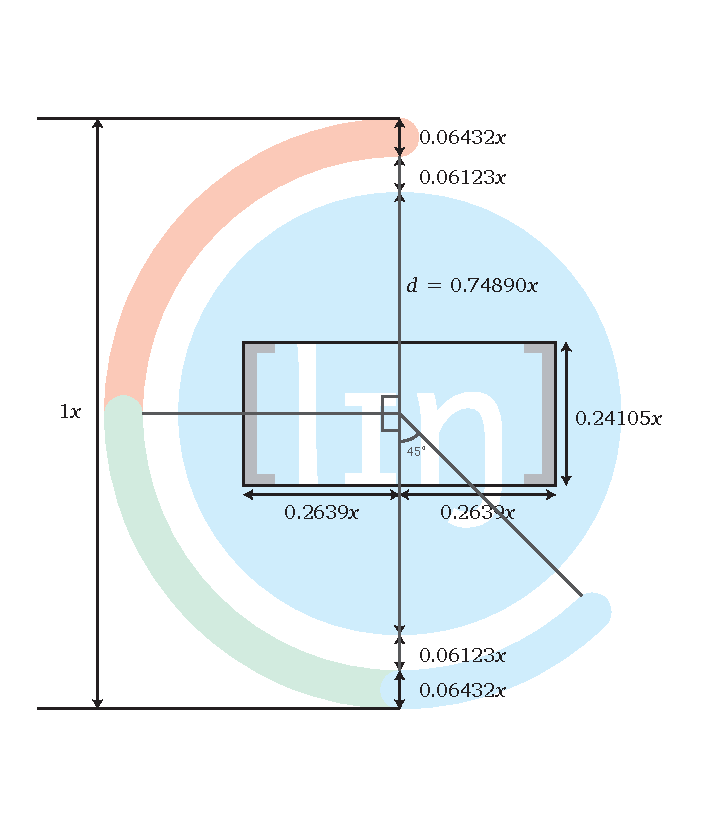
\includegraphics[height=17.5cm]{graphics/logotype_dimensions_2}
		
		
	\end{appendices}
	
	
%	End of document
	\vspace{1cm}
	\begin{center}
		\MakeUppercase{\textbf{-- End --}}
	\end{center}
\end{document}

